\section{Recording CPU Load}
\label{sec:qstat}

Recording the CPU load is executed by a self-programmed tool of Michael Iedema \newline (michael@askozia.com). Its name is
\texttt{qstat} and is available by pressing the \texttt{ESC} key somewhere on the Askozia webpage. Then, in the
``Beta Features'' tab, there is a link referencing to \texttt{debug\_qstat.php}:

\begin{figure} [!ht]
\centering
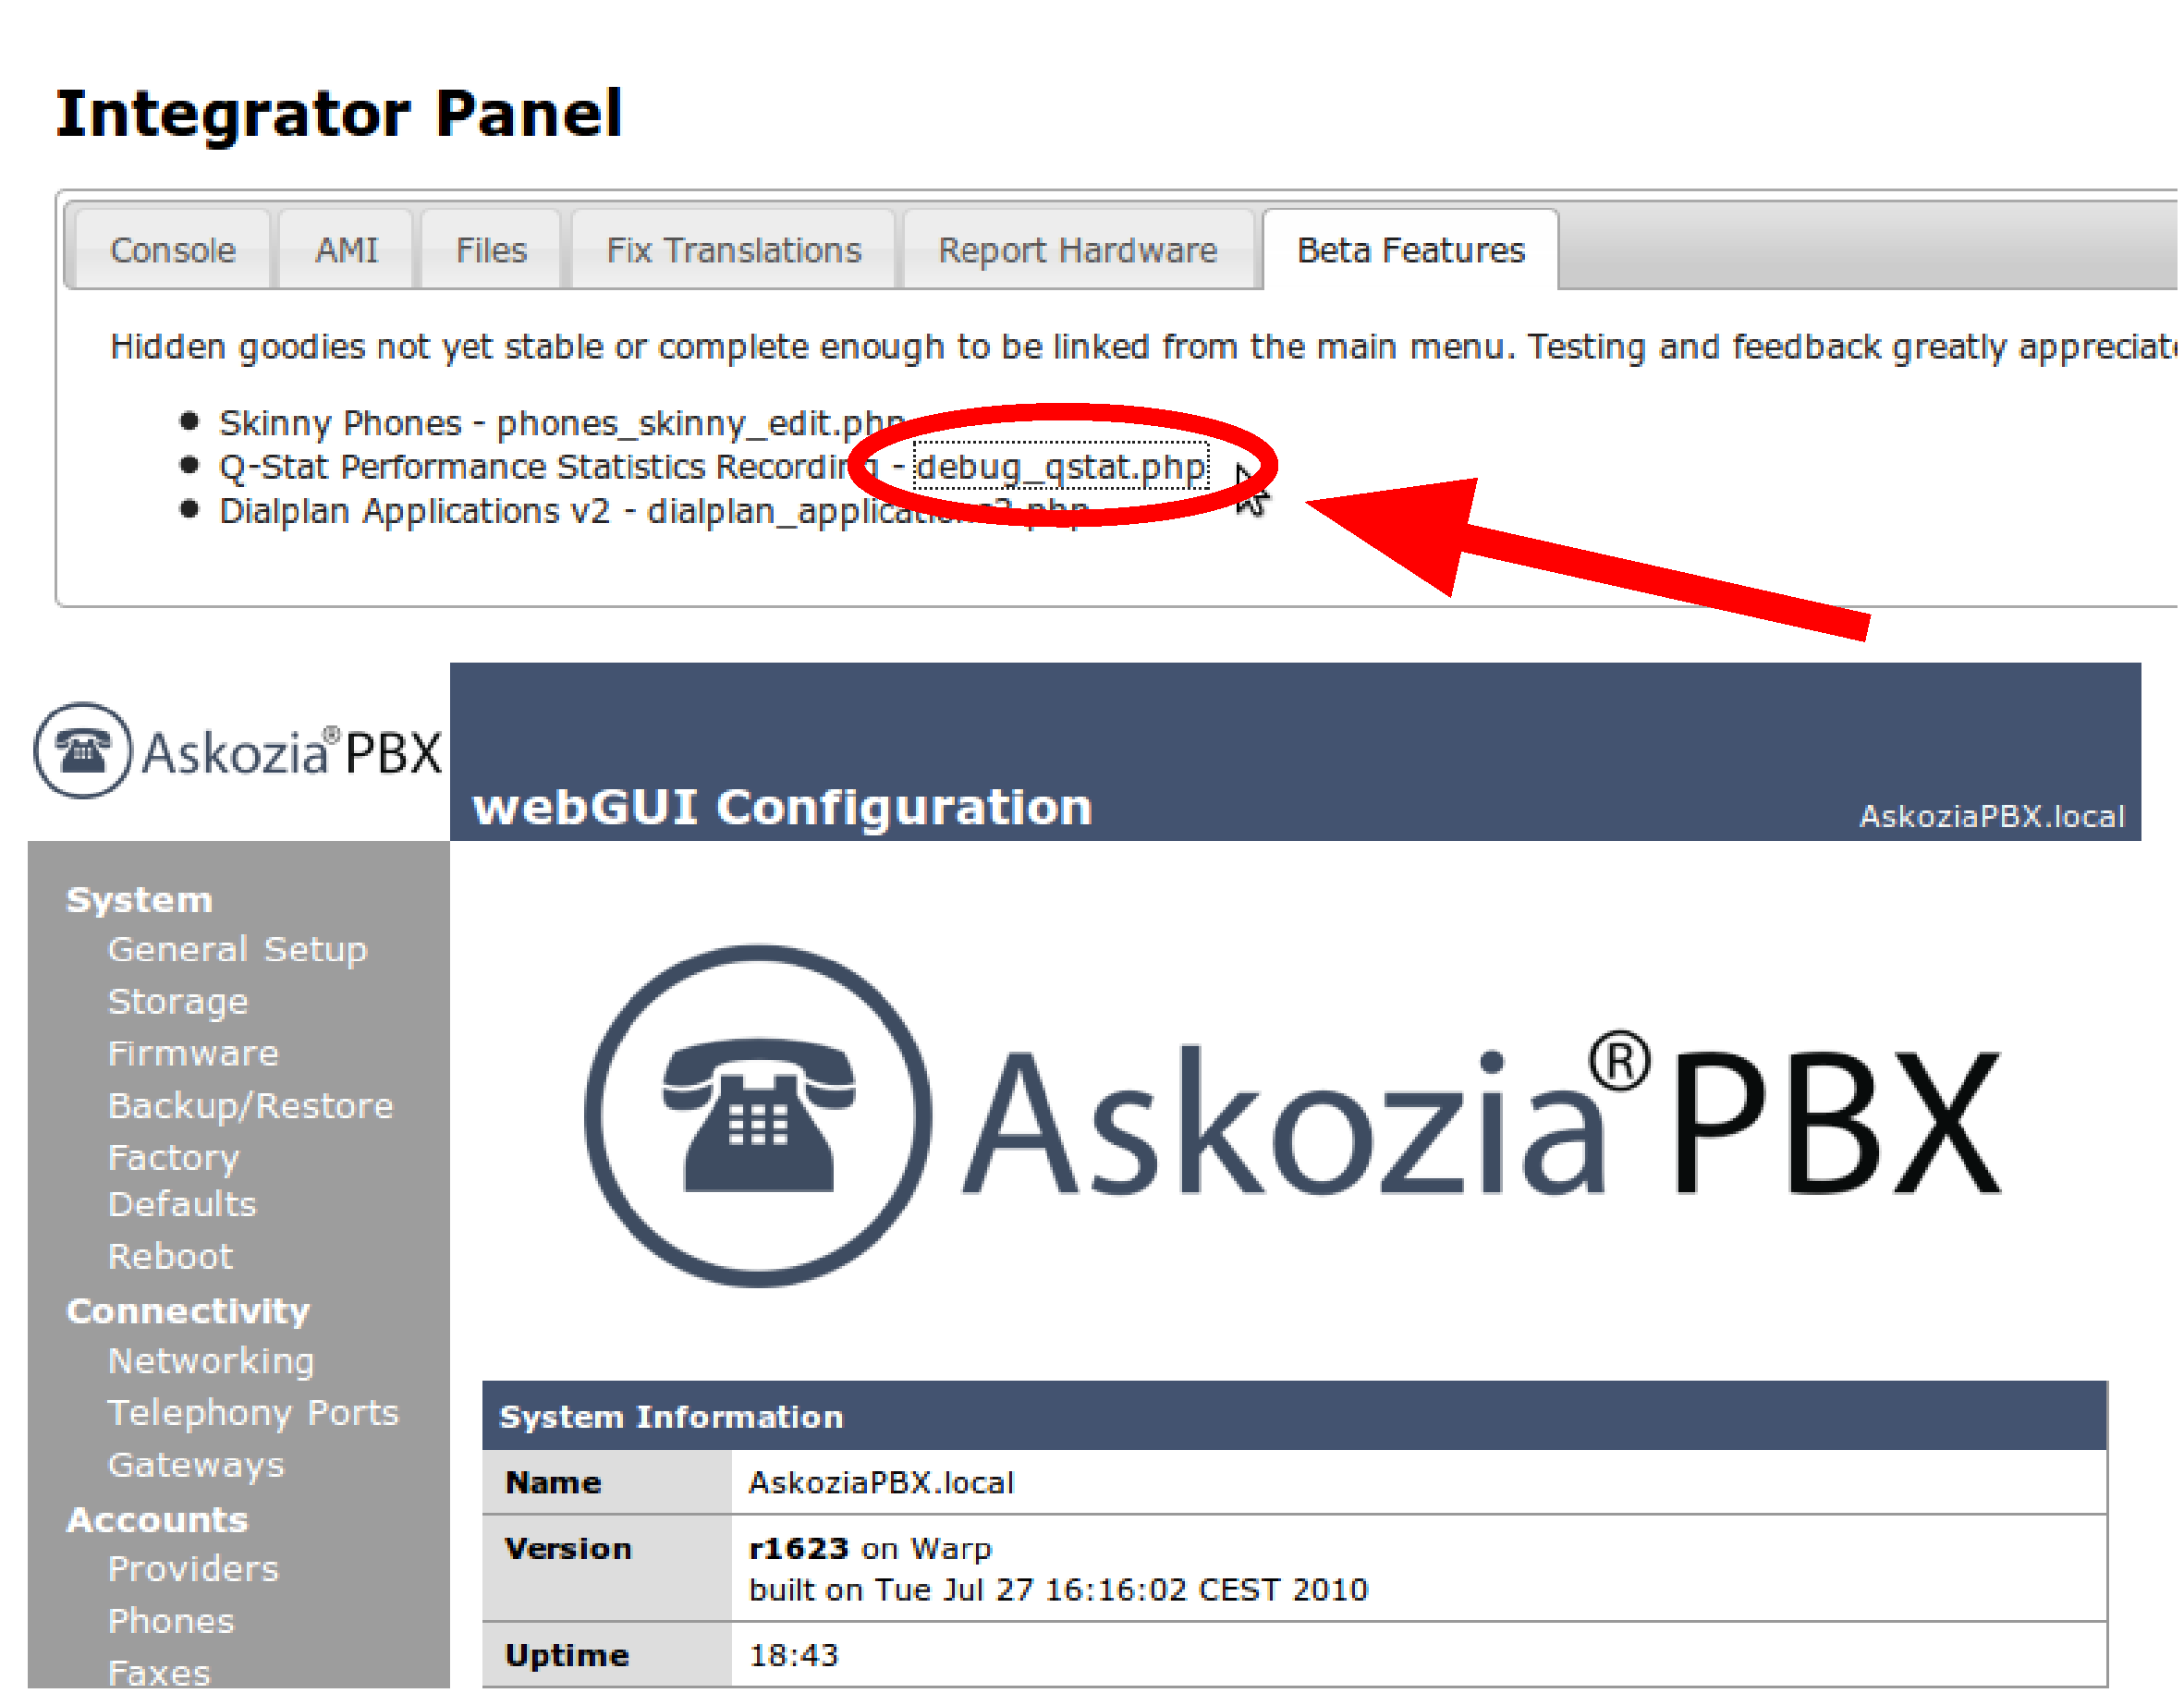
\includegraphics [width=16cm] {qstat-1.pdf}
\caption{Starting qstat manually}
\end{figure}

On the debug qstat page, there is only one button labelled with \texttt{Start}. So, a click on this button starts CPU load
recording by qstat. The button changes top \texttt{Stop} automatically and terminates CPU load recording by clicking on it.
After this, there appears a downloadable file (... .qstat) on the webpage. It contains the recorded qstat data and looks like this:

\newpage
\begin{figure} [!ht]
\centering
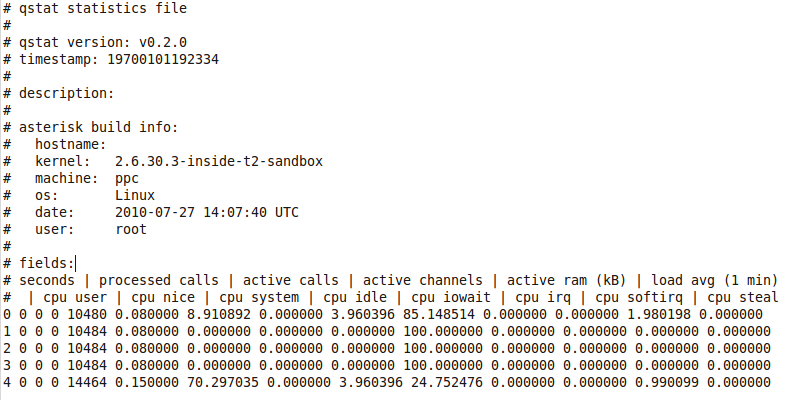
\includegraphics [width=17cm] {qstat-2}
\caption{QStat results}
\label{fig:qstat-output}
\end{figure}

The recorded data comprise multiple CPU load values. The script uses the CPU idle time by subtracting it from 100.
They were verified manually by comparing the qstat values with other values created by using \texttt{top} on the AskoziaPBX.

%%%%%%%%%%%%%%%%%%%%%%%%%%%%%%%%%%%%%%%%%%
\subsection{Starting and stopping qstat}%%
%%%%%%%%%%%%%%%%%%%%%%%%%%%%%%%%%%%%%%%%%%

Of course, the testsuite is not able to control the browser and click on any buttons.
So, the command for starting and stopping qstat is sent manually by using the ajax script.
By mean of this ajax script, it is possible to send bash commands or asterisk commands to the particular process.
This feature is used to activate or deactive recording of the cpu load data by the following command.
It creates a HTTP GET request including the specified interface (\texttt{exec\_ami}: asterisk) and the
command (string between the single quotation marks: \texttt{qstat+start+<description>}).

\begin{lstlisting}[breaklines=true,label=code:qstat-startstop,caption={Starting and stopping qstat recording} ]
$res = $ua->request (GET "http://$ask_ip:$ask_port/cgi-bin/ajax.cgi?exec_ami=%27qstat+start+two-party%27");
$res = $ua->request (GET "http://$ask_ip/cgi-bin/ajax.cgi?exec_ami='qstat+stop'");
\end{lstlisting}

\newpage
%%%%%%%%%%%%%%%%%%%%%%%%%%%%%%%%%%%%%%%%
\subsection{Downloading recorded data}%%
%%%%%%%%%%%%%%%%%%%%%%%%%%%%%%%%%%%%%%%%

For downloading the recorded qstat data, there is a standard \texttt{cat} command of the linux shell used.
As described in the previous section, AskoziaPBX provides a possibility to execute shell commands by web requests.
In contrast to listing \ref{code:qstat-startstop}, the shell interface is used now (\texttt{exec\_shell}: linux bash).
Normally, this command would return all existing qstat files. But before every test, the AskoziaPBX is rebooted and
with every reboot of the AskoziaPBX all qstat files are deleted.
So, it is not possible that there is more than one file - the recorded cpu load data of the last performance test.
The output is shown in figure~\ref{fig:qstat-output}.

\begin{lstlisting}[breaklines=true,label=code:qstat-download,caption={Downloading recorded cpu load data} ]
$res = $ua->request (GET "http://$ask_ip:$ask_port/cgi-bin/ajax.cgi?exec_shell=cat+/var/asterisk/log/qstat/*");
\end{lstlisting}

%%%%%%%%%%%%%%%%%%%%%%%%%%%%%%%%
\subsection{Interpreting data}%%
%%%%%%%%%%%%%%%%%%%%%%%%%%%%%%%%

The measured data are sorted, filtered and shown in a graph.
First, all data of one call (perhaps 1 call) are picked out and sorted. Now, the highest and lowest 25\% of the sorted
data are filtered. So, there are only 50\% of the originally measured values left. This avoids skewed values, because
sometimes there are mean peaks of 0\% or 95\% that are not realistic. This result is called ´´median'' calculation.
The remaining 50\% are averaged and saved in an array at position \texttt{x}, where \texttt{x} is the number of concurrent
calls.

Column A shows the seconds since starting qstat recording. Column B shows the number of concurrent calls.
Column C contains the original measured values of qstat. Column D shows the number of concurrent calls
for the mean values. Column E shows the mean value of the cpu load (100 subtracted by the mean value of the median).
These calculated values are necessary to create a graph like this (figure~\ref{fig:qstat-graph}):

\begin{figure} [!ht]
\centering
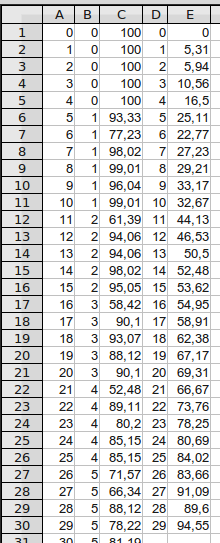
\includegraphics [width=6cm] {qstat-3}
\caption{Original and averaged values of qstat}
\end{figure}

\begin{figure} [!ht]
\centering
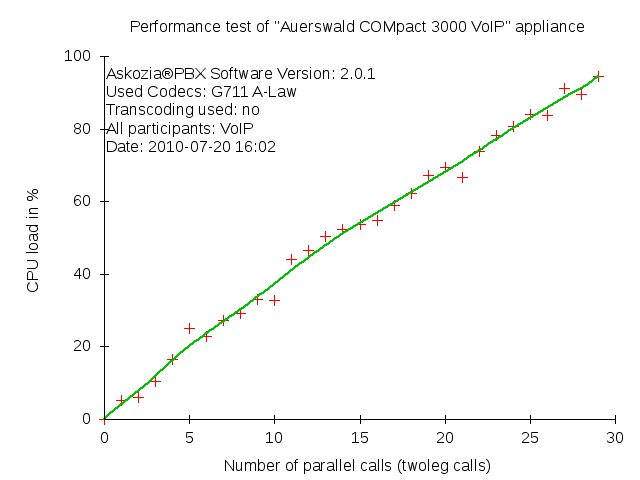
\includegraphics [width=12cm] {qstat-4}
\caption{Graph of the calculated mean values}
\label{fig:qstat-graph}
\end{figure}



